
%TODO Skriv: Sett av 2 dager.

% Diskurs:
% 	- diskuter tid: de fleste neuron med realistisk mengde input vil ha en input per tidsiter. Dette gir at de antagligvis MAKS får eit input per andre iter (dersom alle fyrer maksrate..)
% 		Også da vil det bli meir effektiv modell for tid, men virkelige nytten kommer nok med KANN: da kan vi nok ha 'abituary size' på tidssteget (vil ikkje innføre meir belastning (FOR STATISKE NETT(nett med statisk aktivitetsnivå)) )
% 		JEJE..
%
% 	- avviket mellom SN og KN etter synapse når synapse var skjempestor   (nei: dette er resultat og comparison= 
% 
% 

% 	xxx Skriv grunnen til at eg ikkje har nokon uventede resultater: at dette i all hovedsak har vert en utviklingsprosess, og alle uventede resultater har blitt ordnet på undervegs.
% 		Eksemper på slike er den lange diskusjonen tidligere, om avviket mellom K_auron og s_auron. Dette ble fikset. Mye tid har dermed blitt brukt på dette prosjektet.

% 	TODO TODO Poengter at synaptic transmission matematikk er basert på 2.gen. ANN (mens mykje anna er basert på 3.g). Dette kan diskuteres frem og tilbake!



%todo : analyser avviket fra KN til SN sine depolrarisasjonskurver. Kvifor finnes dette avviket? Kva er greia? Lag mikroplott for stigende og synkende flanke. osv.

%TODO : Skriv at selv om vi ikkje har fått tid til å kjøre effektivitetssammenligning, så har vi funnet eit viktig resultat. KN kan brukes til å oversette mellom 2.gen og 3.gen ANN.
% 		TODO Finn ut korleis 1.gen funker, og skriv evt. inn dette også. (sjå % ref_123@i_KANN i implementasjon_KANN.tex) EVT ikkje nevn "each of the other generation ANN" og "first gen. ANN" fra linja "% ref_123@i_KANN" står på.


% Videre arbeid:
% 	- Lage syn. p.
% 	- Innføre dynamisk teskel (bedre modell for refraction time)
% 	- Foreta effektivitetsanalyse.
% 	- Lage transduction mellom KN og SN. Også mellom fN og KN. Kanskje heile veien, mellom alle generasjoner ANN.
% 	- Utvikle KANN for seg selv. Slik at dette blir så effektivt som mulig..
%
%
%



% Oppsummering (conclution):
% 	innlede med kva som er  gjordt i dette prosjektet (gå gjennom kapittela og skriv ned..)
% 	- Skriv om transduction mellom ANN av ulike generasjoner. Kan bruke KANN til dette! (sjå sec \subsection{The Activity Variable} ).
% 	- Skriv at eg har gjordt den tidsvariante responsen til en overføring (at overføring skjer/ikkje skjer er avhengig av verdi før overføring. Dette skaper eit system som er avhengig av input-historie og tid(lekkasje).
% 		Om til: å ikkje lenger være tidsvariant. Kappa er på en måte tatt utafor tid. Kappa som overført variabel er ikkje tidsvariant, ikkje variant med andre variabler.
% 		=> Den tar vekk ulineariteten innført fra mekanismen: fyring!
%


% Feil/Mangler i denne sammenligninga:
% 	- Har ikkje sett på nettverkseffekta av tidspunkt for propagering av Kappa. Kan bli veldig rart at den propagerer "med en gang" (etter 'current' time iteration).
% 		%TODO analyser dette i diskurs!
% 	- Burde kanskje brukt meir tid på rapporten.
%
%
%
%
%



\chapter{FRA GAMMEL comparison and results -- fil:}


Skrive innledning: Kva er felles for de to implementasjonane: Kva er kjendt i biologien, og kva er utelatt for desse implementasjonene?

Kva har dette til felles med andre implementasjoner, og kva er gjort bedre i denne impelementasjonen i forhold til andre varianter av ANN (1. gen., 2. gen. og 3.gen. ANN).

\section{Forskjell i implementasjon}
Skrive at forskjellen mellom gamle og nye varianten av 3.gen. ANN (SANN) har mykje til felles med forskjellane mellom Moore vs. Mealy Auromata.

Den gamle varianten er for så vidt den som er mest intuitiv å implementere / designe. Denne ser på umiddelbar tilstand (depol. verdi) for nodene. Dersom denne depol. kommer over terskel vil noden gi output til alle sine utnoder.
Dette er en direkte simulering av det biologiske neuronet. Kan beskrives (direkte?) med Moore Automata.

For den foreslåtte varianten vil Mealy automata beskrive systemet bedre. Her er det 'state' for noden og i tillegg input som gir ut-oppførselen.
[skriv kva "utoppførsel" betyr. Alltid samme output (før synapsen) for den Moore-Automata varianten av SANN. For Mealy variant vil output være en flyttallsvariabel]
[skriv kvifor denne tanken kom -- at enkel kraftig prosessor vil være oppmot like effektiv med større flyttalsoperasjoner som ved enkle boolske transmissjoner (tjaneei..)
Dersom vi har mulighet er ferre større operasjoner bedre for den serielle CPU enn mange små operasjoner.]

[Skriv at implementasjonen viste seg å bli meir omfattende enn først tenkt. Skriv om pEstimatedTaskTime og anna ekstra tidsplanlegging]




\section{Testoppsett for sammenligning av KANN og SANN}
Skrive at design av/teorien bak  de to impelmentasjonene er så forsjellig at det er vanskelig å sammenligne de to. En enkel kjøring vil ha statisk input (ikkje-endrende input).
Mealy varianten av SANN (KANN) er spesialisert for ANN med dynamisk (endrende) input. Vil gi eit vanskeligere testoppsett for sammenligning av de to. Lett å implementere for KANN, vanskeligere å implementere for SANN.
(Da må eg ha egene sensor-neuron som er spesiallaga for å sense en slik dynamisk state).

	\subsection{Fleire testoppsett? Beskriv de ulike oppsetta, og kvifor!}
	\subsection{Teste for oppdelte nett: med koblinger med lite overføring/endring i overføring}

\section{Skrive kva som er utelatt} % Kanskje heller i discussion?
Kva var originalt planlagt, men viste seg å bli for mykje arbeid?

\begin{itemize}
 	\item Synaptisk plastisitet.
\end{itemize}



%TODO Flytt denne tilbake til KANN: det er en aktiv del av implementering. I starten av avsnittet: skriv kvifor eg valte å ha den under design og implementasjon: at det er en aktiv del av utviklinga.
% 		I tillegg finner vi trunctation error: dette blir viktig i diskurs! Kan dermed avslutte å snakke om det i dette kapittelet, og ta det igjen (overraskende) i diskurs--biten:
% 			Det eg tenker på er opdagelsen av at SANN har trunctation error, og at denne vil vakse mot infty.
% 			Diskuter, men end opp med at feilen er liten, og vil ikkje være dødelig..
\section{Comparison between the transient time course of the depolarization of the K auron and s auron ,   Vettafaen kor det skal ligge}
To compare %the implementation of (?)
			the two models, we will start with comparing the depolarization of a single node from each model.
The same input to the two nodes should optimally give the same transient time course of the depolarization.

Because of the complexity of each node in a neural network, we cannot use a network of neurons to generate an equal input to the analyzed neuron. 
At least not before we now that they give the same output.
My solution for this is 
%The solution for this was
						to devise an own underclass K\_sensor\_auron for the $\kappa$ANN model and s\_sensor\_auron for the SANN model, that gives an output based on some ``sensor function''.
This sensor function can be made to give an output appropriate for comparing the variants of the node.

Both sensor classes are constructed by sending a function pointer into the constructor of the object. 

\begin{lstlisting}
K_sensor_auron::K_sensor_auron(
  std::string sNavn_Arg, double (*pFunk_arg)(void) ) 
     :  K_auron(sNavn_Arg)
{
	// Assign the sensor function:
	pSensorFunction = pFunk_arg;
	// Add to pAllSensorAurons list:
	pAllSensorAurons.push_back(this);

	...
}
\end{lstlisting}

Where the member variable \emph{double \mbox{(*pSensorFunction)(void);}} is a function pointer that is assigned the the function pointer adress that is sent in as an argument in the class constructor.
%This causes \emph{pSensorFunction} for point to the function sent in as an argument in the constructor.'
The variable pAllSensorAurons is a list containing all the valid sensor objects, used for updating the value of each sensor neuron when \emph{time\_class::doTask()} iterates time. %i time_class::doTask()

\begin{figure}[hbtp!]
	\centering
	%\begin{center}
		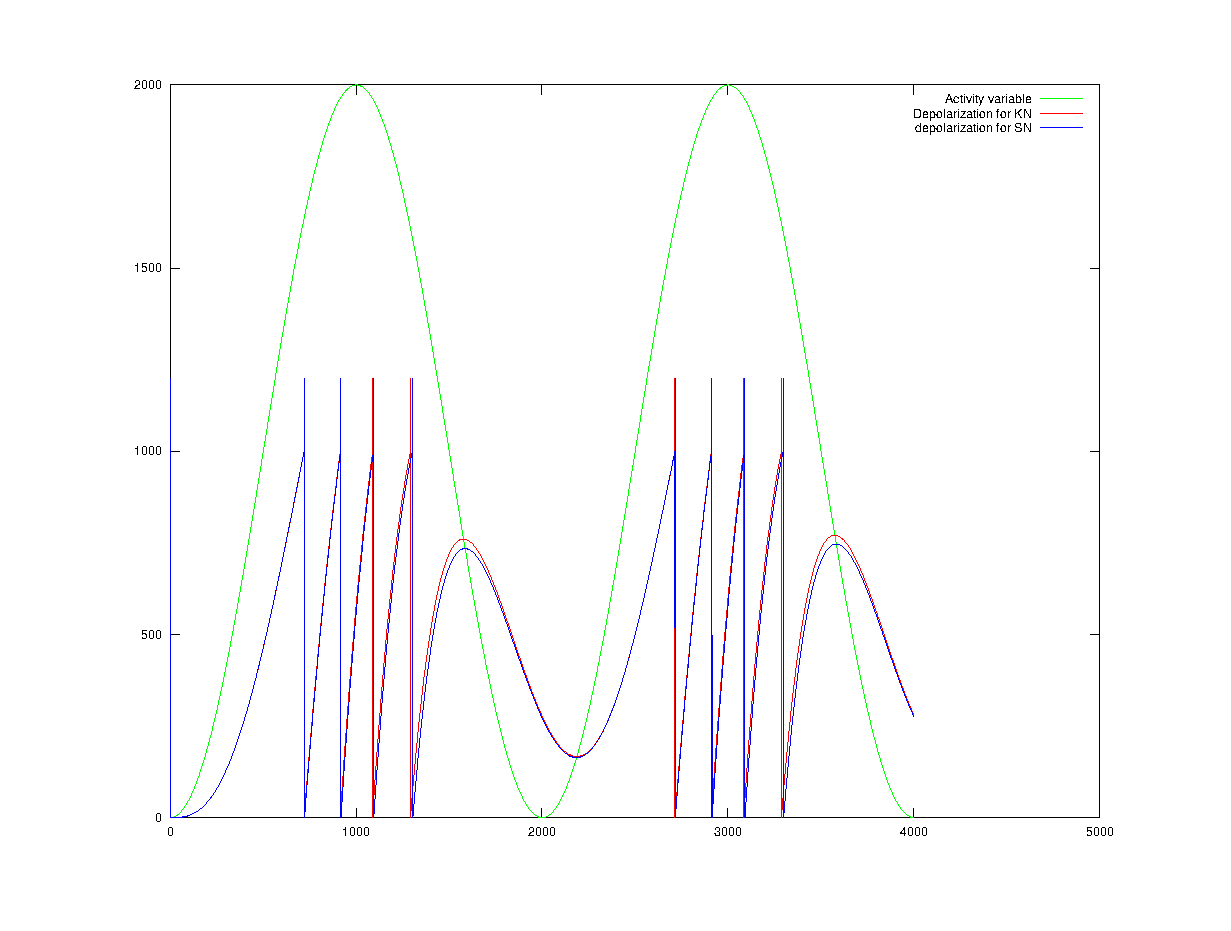
\includegraphics[width=0.95\textwidth]{eps_Comparison_between_the_two_sensors__depol.eps}
	%\end{center}
	\caption{The depolarization curve for a SANN node and a $\kappa$ANN node with the same input. The sensor function is also plotted in green for the analysis of the result.}
	\label{figComparisonBetweenSsensorAndKsensorDepolCurve}
\end{figure}

%The sensor function used for the comparison of the time course of the depolarization of a single node is 
The sensor function used in fig. \ref{figComparisonBetweenSsensorAndKsensorDepolCurve} has the formula \mbox{$f(t) = \tau (1 + cos( \frac{\pi \, t}{1000} ))$}, where $\tau$ is the firing threshold for the neuron. 
The activity variable of the K\_sensor\_auron is set to the value of the sensor funciton every time we iterate time. %XXX i time_class::doTask() Skriv litt meir. 
%For the K\_auron the activity variable is at each time step set to this variable. 
When \emph{time\_class::doTask()} updates the K\_sensor\_auron's activation level, this is done by updating the ``input'' to the dendrite.
%When K\_sensor\_auron changes its activation level, we do this by sending the sensed signal to the dendrite. 
%TODO Neste linje: referer (cite) eller internreferer til annen plass i teksten. Trur det er best å CITE.
This is very simular to the mechanisms of a sensor neuron in biology. %Evt kan eg skrive at "this is strongly inspired by nature".
%referer.
%Beste for refereringa over er nok å skrive om dette i BiologiskeSystemer.tex, og referere til plassen det står. 

%TODO Skriv ENTEN forrige linje ELLER neste greiene. NO: Repeterer meg sjølv! XXX
This implementation is strongly inspired by the biological neural system, and the stimuli is sent to the dendrite as any synaptic input.
For the K\_sensor\_auron this gives the code
%TODO Vær sikker på at dLastSensedValue = dSensedValue; dSensedValue = (*pSensorFunction)();
% Først i koden, under.
%ELLER kanskje heller: skriv om changeKappa_abs() ?!?
\begin{lstlisting}
dLastSensedValue = dSensedValue;
dSensedValue = (*pSensorFunction)();

changeKappa( dSensedValue - dLastSensedValue ); 
\end{lstlisting} %Eller så kan vi gjøre det direkte. (sette Kappa til målt verdi. har impa begge..)
and for the s\_auron we have %TODO BLI HEILT SIKKER PÅ ALPHA. Sjekk om det fortsatt er som under, eller om dette har blitt tatt inn i s_dendrite::newSignal() XXX
\begin{lstlisting}
pInputDendrite->newInputSignal( (*pSensorFunction)() );  
\end{lstlisting} % TODO Forstå greia med ALPHA! (er der fortsatt slik at eg sender inn
							% pInputDendrite->newInputSignal( (*pSensorFunction)() * ALPHA );   XXX ?


Because of the mechanisms implemented for synaptic transmission in $\kappa$ANN is based on the derived, we change $\kappa$ by the discrete variant of the derived; 
The current sensed value minus the last sensed value.% or dSensedValue - dLastSensedValue.
For the s\_auron we incoorporate the time constant T as $\frac{1}{T} = \alpha$ %eller :  $.. = $ ALPHA 
		by sending the above listed input to the s\_sensor\_auron's dendrite.


In figure \ref{figComparisonBetweenSsensorAndKsensorDepolCurve} we can se the results. 
As can be seen, the depolarization of the K\_auron and the s\_auron is quite simular.
There is a small difference between the curves.
%It is hard to know the specific reason for the error in this implementation.  In the following section I will discuss possible explanations.

What is interesting about this curve is that it seems that the depolarization curves follow eachother exactly %Dette er rett stavemåte: exactly (google translate)
for the rising phase of the sensor curve. For the falling phase of the curve we get some difference between the depolarization of the SN and the $\kappa$N.

% Skrive at for SANN så:
For discrete integration we may get something called the trunctation error. The ``local truncation error'' is the immediate error after each time step. 
The ``global truncation error'' is the error following integration multiple local truncation errors. %eller "many truncation errors", eller noke anna? (kan bli for pent språk også!)
The global truncation error is defined as the absolute difference between the approximated solution and the actual solution. 
For the SN this might become a problem, and could be the basis of the difference of the simulated node's depolarization.%Skriv om. XXX

% TODO TODO TODO Skriv også at denne "truncation error" er tatt hand om i KANN, og bude vore minimal. For SANN er ikkje dette mulig (Ingen mulighet å rekalulere verdien).
%  					XXX Dette er veldig viktig poeng for seinere analyse av KANN vs. SANN!




	\subsection{Trunctation error of the SN} %Kanskje skrive "Spiking Node". Hugs at overskrifta blir også oppført i "index".
	\label{ssecTruncationErrorOfSN}
In SANN each node is modelled as a leaky-integrate-and-fire neuron.
When the depolarization of the SN is updated, the leak of the neuron calculated as the previous value times the leak constant.
The updated value then becomes %todo Skriv om denne setninga.
\begin{equation} %TODO Introduser denne ligninga tidligare i oppgava. Her skal eg bare skrive siste del av den:    v_t = (1-\alpha) * v_{t-1}  XXX HAR EG GJORT DET? TODO SJEKK!
	v_t =  (1-\alpha) \cdot v_{t-1}  
\end{equation}
%TODO Skriv om: krøtkete måte med/mellom alle komma'ane.
The discretization of the system introduces a small error, the local truncation error, that varies with the size of the time step and the derived of the value function $\dot{v}(t)$. %"local truncation error"

The leak is calculated as the $-\alpha v_{t-1}$.
% Skriv at når feilen oppstår, så er dot(v(t)) positiv, dette gir:
When $\dot{v}(t)$ is positive, $v_{t-1}$ is less than the value $v_t$, varying with the size of the time step and the differentiated value function $\dot{v}(t)$.
When $\dot{v}(t)$ is negative, we get the oposite result.
%skriv at dette nuller ut problemet. (MEN (det kommer at) siden det alltid fyrer etter positiv flanke, blir det integral av en liten integralfeil ved kvar fyring. XXX Viktig poeng. Sjekk at det er stort nok skrevet lenger nede.

Each small error is integrated up to a larger error, the global trunction error. 
If some situation is analyzed where the value is the same as the initial value, the integral of the derived over this interval is per definition zero.
Global trunctation error will then dissapear. 
This further implies that for a continous signal that varies around some working point, the global trunctation error will not diverge.  %google sa at det heite "diverge"

\begin{figure}[hbt!]
	\centering
	%\begin{center}
		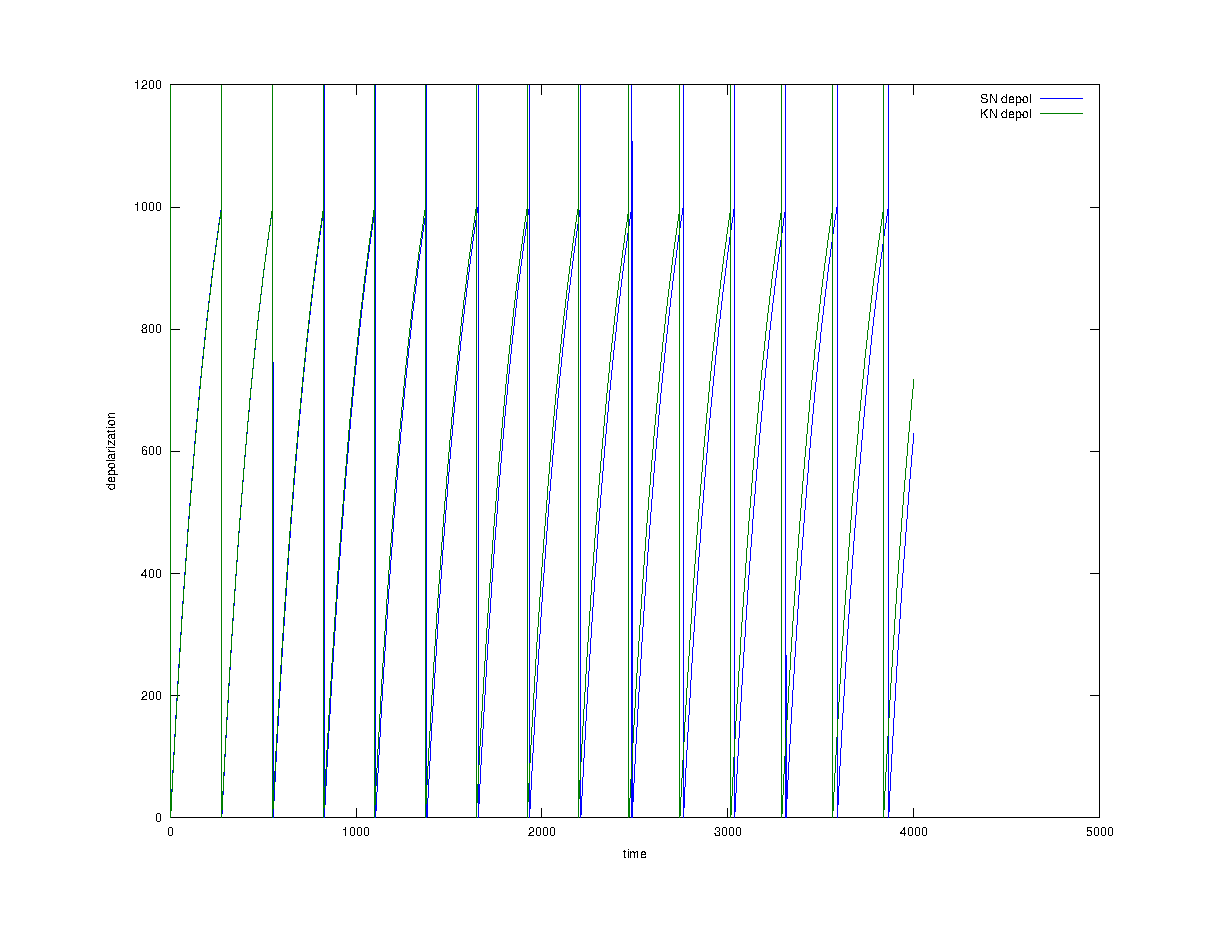
\includegraphics[width=0.95\textwidth]{eps_comparison_between_KN_and_SN_ConstKappa.eps}
	%\end{center}
	\caption{The depolarization curve for a SANN node and a $\kappa$ANN node with the same input. The sensor function has an input equivalent to an activation level of $\kappa = 1.5 \tau$ for both nodes.} %XXX Eller for begge nodeModeller
	\label{figComparisonBetweenSsensorAndKsensorDepolCurveCONStActivityLevel}
\end{figure}

The depolarization of a neuron have a discontinuity when the neuron fires an action potential. 
When the neurons depolarization reaches the firing threshold the value is reset to $v_0 = 0$.
In other words, each time the value of a node reaches a positive threshold, the value is reset.
In this case the global trunctation error will continue to grow, and the difference between the value curves for the SN and the $\kappa$N continues to grow. %TODO Ikkje dette. Skriv heller eit utfall som Stavdahl vil syns er SKUMMELT!

To se if this is the backgound for the error, we isolate the error by giving the sensor aurons a constant sensor function, with an activation level of $\kappa = 1.5 \tau$.

The result is presented in fig. \ref{figComparisonBetweenSsensorAndKsensorDepolCurveCONStActivityLevel}. % .eps
If the previous analysis of the problem is sound, the SN should have a depolarization that is higher than is should be.
This implies than the depolarization curve for the SN would be ``before'' that of the $\kappa$N, which is the opposite of the situation of fig. \ref{figComparisonBetweenSsensorAndKsensorDepolCurveCONStActivityLevel}.





	\subsection{Rounding errors}
%TODO Skriv om: Ikkje røp løysing først. La det være litt spenning!
After a more thorough analysis of the error, it seems that the difference is an effect of a rounding error.

If we change wievpoint on the error and see the difference between the two cuves as an effect of time, we can say that the $\kappa$N's depolarization curve lies before the SN's depolarization curve.
This implies that the $\kappa$N fires before the SN, and thus starts earlier on the depolarization for the next period.

In many programming languages a float is always ``rounded down''. This means that the DECIMAL %XXX FINN RETT ORD: Det som står etter komma TODO
	is removed from the number, and the integer becomes the same as the integer part of the number.

%TODO Viktig: Hugs å skrive om kvifor eg valte en mindre periode i starten av sensor-funk. Dette er viktig, ellers trur han nok at eg bruker dette for å skjule feilen..
\begin{figure}[hb!tp]
	\centering
		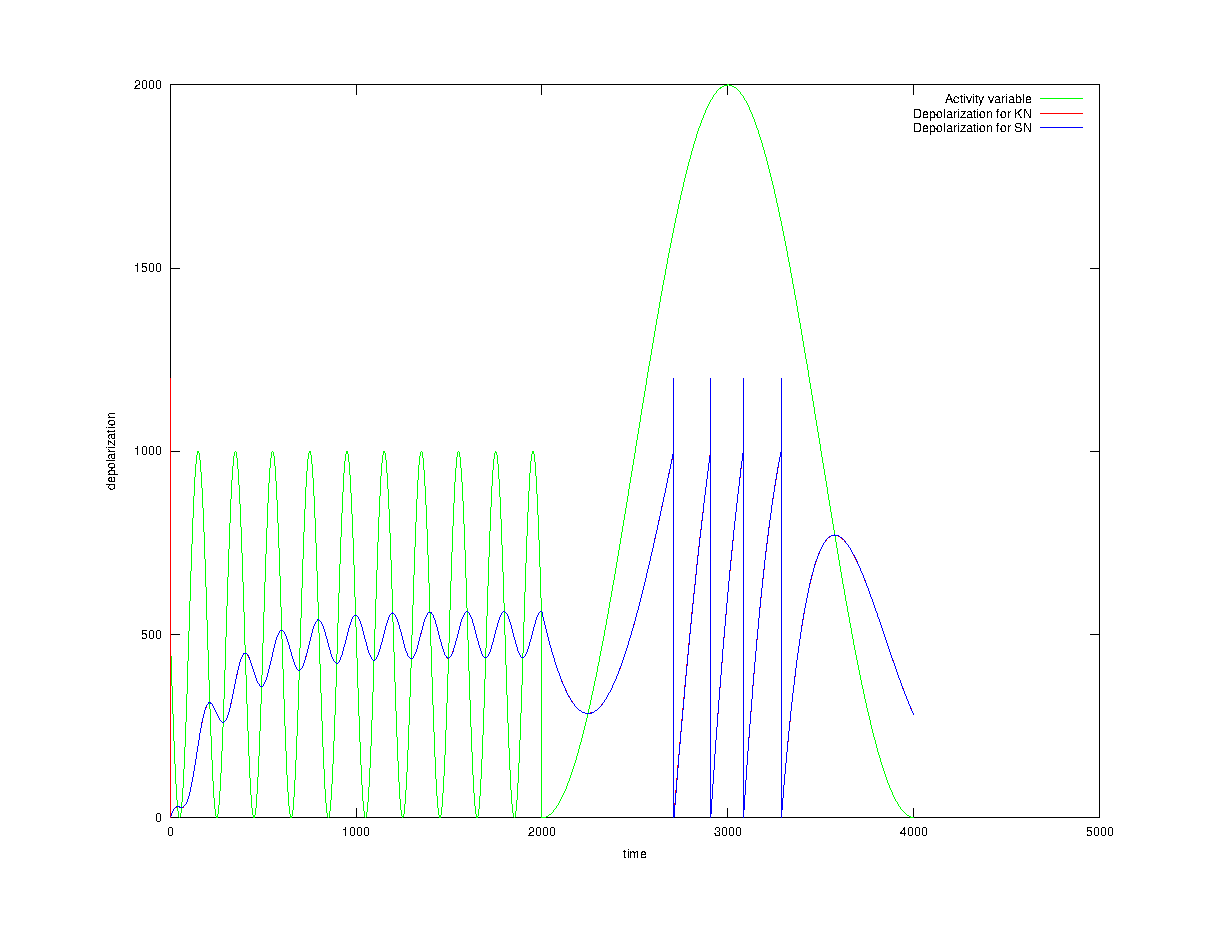
\includegraphics[width=0.95\textwidth]{eps_Comparison_between_the_two_sensors__depol_FIKSA.eps}
	\caption{Comparison between the SN's and $\kappa$N's depolarization curve. The sensor function is plotted in green for analysis purposes.}
	\label{figComparisonBetweenSsensorAndKsensorDepolCurveFIXEdError}
\end{figure}

When the $\kappa$N calculates the estimated firing time, this calculation is done in a double precision floating point number. 
To use this in the scheduler is must first be transformed to an integer variable. When this time step arrives, the task is executed.

%TODO Skriv at vi vil heller runde til nermeste integer, opp om det er best.
% Så skriv korleis dette gjøres, så finn rett kurve.
% TODO analyser frem og tilbake om kor feilen ligger. Det er fortsatt mulig at feilen er for KANN (men trur ikkje det. Legg at feilen er maks når subthreshold polarization er størst. Osv.) XXX
If we instead round to the closest integer, by adding $0.5$ to the float before it is converted into an integer, we get the depolarization curve presented in fig. \ref{figComparisonBetweenSsensorAndKsensorDepolCurveFIXEdError}.
In the improved depolarization curves for the auron, the error is small and can not be seen on the plot.

%Ikkje heilt sikker på om det er heilt rett: størst etter "rising flank of the ..", Bli heilt sikker på dette.
The error is found to be largest right after the rising flank of the activity variable's curve. %TODO ta vekk:   [ , the value of the sensor function. ] ?
For the situation in fig. \ref{figComparisonBetweenSsensorAndKsensorDepolCurveFIXEdError} this is at time t=3000.
At this time iteration the value of the SN is 1.015 more than the value of the $\kappa$N. 

This deviation is substantially smaller that the deviation originating from the rounding error, but it indicates that the analysis made in the previous subsection is correct. %gjør om: ikkje "correct" men kanskje mindre påståelig?
%TODO Skriv analyse av denne feilen, og peik på mulige scenarioer.


% TODO KANSKJE :   \subsection{Floating point calculation pitfalls}
%                  Skriv om mulighetene for feil når man bruker float/double.


% - integralfeil for SN
% - Integralfeilen kommer antagelig av at lekkasjen  
% - For SN vil lekkasjen regnes ut fra verdien ved forrige tissteg. Denne diskretiseringseffekten vil forplante seg i at for positiv derivert av depol-kurva vil SN-depol være litt over, og for negativ flanke : motsatt.
% 		Dette er fordi lekkasjen regnes ut fra forrige verdi, som for stigende flanke er mindre enn den noværande verdien, og vi får en mindre lekkasje => for stor verdi.
% - denne feilen vil nulles ut for eit periodisk signal uten sprang (over en periode vil integralet av positiv flanke og neg. flanke bli null.
% - dersom vi har eit sprang, eller enda verre: eit sprang som alltid ligger etter en viss mengde med pos. flanke, vil vi få summert opp integral-feilen.
% For auronet vil depol settes lik 0 etter en viss mendge pos. flanke for depol. kurva. Dette skaper problemet.

% Eg har også vurdert om det er feil fra implemenasjonen: at de har ulik refraction time, MEN eg trur ikkje dette: 
% 		En slik feil ville vore mindre (eit-to tidssteg per fyring) => ikkje synlig på eit plott over fleire tusen iter's.

% Den lille forskjellen mellom s_sensor_auron og K_sensor_auron er noko eg kan skrive mykje om i 'discussion'.
% Eg har tanker om at det er pga. at eg bruker integer (tid) i ligningene, og vi får dermed avrundingsfeil. Litt overraska over at feilen er så liten..
% 	Det er også mulig at den lille forskjellen kommer av forskellane i korleis sensor-funksjonen blir oversatt til depol.
% 		- K_sensor_auron oversetter sensorFunk direkte til aktivitetsVariabel Kappa, mens
% 		- s_sensor_auron sender gir eit enkelt input per tidsiterasjon gitt av ligninga (W_ij / [time constant]), eller  ALPHA * W_ij
%   XXX Dette trenger grundigare analyser!

% Svaret var: avrundingsfeil av casting fra float til unsigned (fra estimering av tidssteg til Tidssteg). Dette ble alltid runda ned. Løste ved å +0.5 før casting. Funker drita bra!





%XXX Skriv i conclusion:
%Because a network of connected neurons have a large degree of complexity, it is best to start with comparing the depolarization of single nodes.
%For comparison of the two models, we will first compare the depolarization of a single neuron of each model.
%Because a system comprised of a network of neurons have 

%IKKJE TA MED. Er ikkje heilt sikker på kvifor det er slik. Dersom eg skal ha det med, kan eg jobbe med dette når rapporten er ferdig!
%\section{Synaptic Transmission}
%Få heilt klar for deg koleis sammenehenen er mellom K syn.t. og s syn.t. er før dette skrives.
%
%When the comparison between the postsynaptisk depolarization began, it could seem like the equations for synaptic trantmission were wrong. 
%The postsynaptic node of a s\_synapse had a larger value that that of the postsynaptic $\kappa$N in a corresponding $\kappa$ANN circuit.
%After analyzing the result, it was found that the error followed the same principles that were discussed in section \ref{ssecTruncationErrorOfSN}.
%
%The initial testing of the different ANN models use few nodes with a strong connection between them.
%The synaptic connections had a synaptic weight that could make the postsynaptic node go to suprathreshold levels in less then ten transmissions.
%In biological networks and in useful artificial networks, a connection of this size would make the system %XXX XXX DÅRLIG (skriv dette på bedre måte..)
%
%The result of this was that the initial transmission of a SN would cause a jump to this level, and the 
% % TODO dersom eg skal skrive denne secion, så må eg legge ved plot:  ../FDP_ANN/datafiles_for_evaluation/sammenligningEtterSynapseMedKonstantPresynSensorFunk.eps !
%When the circuits were initially



\section{Resultat for effektivitetssammenligning}



\section{Discussion}
In the course of this project what is thought to be a new model for artificial neural networks have been developed. 
Because the primary focus of the project was to compare the developed model for ANN with other ANNs with the ability to represent both firing time and firing frequency, the development and implementation recieved this focus. 
%The new model was therefore initially implemented as a mere variant of a third generation ANN, with respect to information propatation.
Because such a model could not be found, $\kappa$ANN was compared with the model capable of representing firing time, SANN.

The new model was initially implemented as similar to SANN as possible, to make the two models compatible.
This caused the initial implementation of $\kappa$ANN to be a mere variand of SANN, with respect to information propagation;
	The activity of the node propagated when the calculated value of the node went to suprathreshold levels.
%The new model was therefore initially implemented as a mere variant of a third generation ANN, with respect to information propatation.
%Initially, the activity of the nodes propagated when the calculated value of the node went to suprathreshold levels.
%When the model was futher developed, it became clear that  %TODO Skriv når, og kvifor(at da) kappa propagerer.

%If we define the third generation ANN as a network of nodes capable of calculating a state of the node based on past and present input, and by this state deside the firing time of the node, it is possible to places $\kappa$ANN in this group.
%If we define the third generation ANN as a network of nodes capable of integrating the input to a state for the node, and this state gives the firing time of the node, it is possible to place $\kappa$ANN in this group.
%If we define the third generation ANN as a network of nodes capable calculating the state (``depolarization'') for the node, and by this state deside the firing time of the node, it is possible to place $\kappa$ANN in this group.
If we define the third generation ANN as a network of nodes capable of firing a spike as the result of past and present input, $\kappa$ANN could fall under this category.
%If the output of a node is given as a spike following a history that cause the value of the node to go to suprathreshold levels, the implementation would fall under the previous definition of SANN.
An implementation where the output of a node is given as a spike following an imput history that cause the value of the node to go to suprathreshold levels, the implementation would fall under the previous definition of SANN.
%If we define the output of each node in $\kappa$ANN to be the spikes following a history that cause the value of the node to go to suprathreshold levels, the network would fall under the SANN catherory as previously defined.
The nodes of this implementation of $\kappa$ANN could be said to be a Mealey automata of a SN, and could therefore give output to a SN. %SANN model. %BLI HEILT SIKKER PÅ MEALY AUTOMATA! TODO
%This is how it is implemented in this project.

%TODO Enten skriv koleis den propagerer, eller kvifor det faller utafor:
If the third generation ANN is defined as a network of nodes where the activity is propagated by spikes, $\kappa$ANN falls outside this category.
% 																									BEDRE:		input is integrated to ...
%If the third generation ANN is defined as a network of nodes where the activity is propagated with spikes, and the input of a node is integrated to become the value of the node, $\kappa$ANN falls outside this category.
%																											%and a node's value is the integral of its input, $\kappa$ANN falls outside this category.
In all versions of SANN the author has been able to find, synaptic transmission is based on adding the synaptic weight to the postsynaptic node's value. %the input of a node is integrated up to the value of the node.
The value of the node ``leaks'', or looses value as a funciton of time and the value of the node.
If the value goes to suprathreshold levels, the node sends a simulated action potential causing transmission in all its output synapses.
This could be said to be a direct simulation of a LIF neuron.
%This is in other words, quite different than the mechanisms of $\kappa$ANN nodes.

In $\kappa$ANN we have ``firing'' for a different reason, one is to be able to compare the transient time course of the value of the node.
%As firing of a node causes the value to be reset to zero, this is an important part of the inter--spike period for the neuron.
%To be able to simulate this and thus the spike time
%TODO  HER  TODO  HER  TODO  HER  TODO  HER  TODO  HER  TODO  HER  TODO  HER  TODO  HER  TODO  HER  TODO  HER  TODO  HER  TODO
This is done to be able to be able to use mechanisms of learning called STDP, and to be able to communicate with SNs.
If a $\kappa$ANN implementation wants to communicate with a SN, this could be done by defining a special set of transductor synapses.
These synapses would use the synaptic transmission scheme from the SANN model, and ouput would only be sent through it after a spike(after the right time delay).
%sending output through it after a spike (after the right time delay).


%
In this implementation, the time of propagation also differs. It was found best to propagate $\kappa$ ``immediately'', that is the timeiteration after the time of the changed $\kappa$.
Initially the propataion of the activity level waited until the first spike of the node. This gave unrealistic time delays in the network. %TODO Finn/Lag figur! Skriv om dette tidligere!
% TODO TODO TODO TODO TODO TODO TODO TODO TODO TODO TODO TODO TODO TODO TODO TODO TODO TODO TODO TODO TODO TODO TODO TODO TODO TODO TODO TODO TODO TODO TODO TODO TODO TODO TODO TODO TODO TODO TODO TODO TODO TODO TODO TODO 
% TODO Dårlig under her . Litt rotete over også..
% TODO TODO TODO TODO TODO TODO TODO TODO TODO TODO TODO TODO TODO TODO TODO TODO TODO TODO TODO TODO TODO TODO TODO TODO TODO TODO TODO TODO TODO TODO TODO TODO TODO TODO TODO TODO TODO TODO TODO TODO TODO TODO TODO TODO 
%It was found that the time delay introduced by waiting for the first spike gave a delay thought  to be to large. In this implementation the activity of the node propagates as soon as the input value changes.
%
%The $\kappa$N could also give output as a function of the only its input. 
In this case the node becomes stateless in respect to its output, and becomes a variant of the second generation ANN.
The activation function is based on a mechanistic model of the neuron, and differs somewhat to that of a node of a second generation ANN.
%If we instead let each $\kappa$N give an output as a function of the present and estimated future input, and give a similar output, the network becomes something else.
%The output now varies as a function of the input, and the node becomes could be made stateless in this respect. 
%In this case the ANN nodes become very similar to a node of a second generation ANN.
As output of a node is given by the activity level of the node, not the state of the node, we have that the KANN node is able to communicate with an ANN of the second generation.

We still have the oppurtunity to calculate the value of the nodes by the concept of ``time windows''.
By making specialized synapses for this purpose, a $\kappa$N could also communicate with a node of the third generation ANN, SANN.
for the connection between a KN and SN, where only the spike is transmitted, the model makes it possible to communicate with a SANN node. 

%If desired, the spike time and state of the neuron can still be calculated. 

In this implementation, it is possible that the full advantage of the new model is neglected in the desire to compare the model to the SANN model.
Because this was first discovered when the results were analyzed, and due to little time, this will be placed under "for furter work". % TODO TA vekk/SKriv om!
%FORTSETT HER!

%så gå over til sammenligning av denne mot SANN.



\section{Discussion 2. Denne skal nok vekk.}

% TODO TODO TODO TODO TODO TODO TODO TODO TODO TODO TODO TODO TODO TODO TODO TODO TODO TODO TODO TODO TODO TODO TODO TODO TODO TODO TODO TODO TODO TODO TODO TODO TODO 
% DETTE er ikkje diskussjon. Dette er implementasjon eller noke.      TODO FLYTT TIL design-kapittel. Siste section: discussion (eller noke)
% TODO TODO TODO TODO TODO TODO TODO TODO TODO TODO TODO TODO TODO TODO TODO TODO TODO TODO TODO TODO TODO TODO TODO TODO TODO TODO TODO TODO TODO TODO TODO TODO TODO 

%En eller anna plass: (ikkje akkurat her) Skriver her fordi eg har inspirasjon no, og ikkje vil leite..) 	Ja! Kanskje i "conclutions"XXX
Implementing the mechanisms of a neural simulator is not trivial, even without optimizing it for run time efficiency.
%todo SKriv om neste linje! xxx
Even if this is not an important aspect of this project I have tried to, wherever possible, optimize the implementation for efficiency.
%Skrive kvifor: Om at designet er optimalisert både for generalitet (for å gjøre utvidelser/endring lettere) og for effektivitet. DETTE for å kunne bruke implementationen videre (personlig, eller for andre).

The functions that are most often called are inlined. This means that I have given a hint to the compiler to put the compiled code wherever the functions are called.
This causes the function calls to run faster but also increases the size of the executable file, so this should be used with caution. %Kanskje skrive dette, men også da skrive størrelse på endelig program. ca. 0.5 M (?)
For this implementation, size will not be a problem. %Kvifor?
Inlining of functions are still kept to a minimum, in case of further work on this software. %skriv annaleis. Kvifor "in case of further work on this software."? Forklar bedre, eller skriv om (anna argumentering).

Also in other parts of the implementation, the code is written with a focus on possible future expantion.
%Difor er ting laga enkel å forstå for en som kan nevro: oppsettet av nodene er lagt opp som det biologiske neuronet.
The object model is designed to be general for the two models, both to make the two implementations more comparable for this project and to make the implementation better suitable for future comparison.

The design of each node is based on the biological neuron to be more intuitive for programmers with knowledge of neuroscience. 
This is not only to make the implementation easier to use for potential future programmers, but also because little is known about what is important in neuroscience.
If the implementation is constructed strongly inspired by the emulated system, with multible elements constructed in the same way as the original system, expantion and modification of the indivitual elements involve less effort.
Say, for example, that new aspects are discovered tomorrow. In this case, the code can easier be modified after this discovery.

This principle does not only account for future uses by other programmers.
In multiple occations, aspects that are where new to me have been implemented at after the main functionality of the classes where designed. 
This required less work because I followed principles that was important to Bjarne Stroustrup during the creation of C++; To make the design general and open and suited for any future uses.%ELLER NOKE Siter"TheDesignAndEvolution of C++".


% TODO TODO TODO TODO TODO TODO TODO TODO TODO TODO TODO TODO TODO TODO TODO TODO TODO TODO TODO TODO TODO TODO TODO TODO TODO TODO TODO TODO TODO TODO TODO TODO TODO 
% dette ER diskurs (?) :
One element that is not implemented, is axo--somatic and axo--axonic synases. 
This is synapses where the input to the postsynaptic neuron enters at other places of the neuron than the dendrite. 
In biology, most inhibitory synases have theire input close to the soma of the postsynaptic neuron. 
This will give the inhibitory input less delay compared to the exitatory input, and might be an important aspect in neural computations.
This can be implemented easily if this is found to be important for some future use of this code.

An other important aspect that is not impelented is axo-axonic synapses, linked to short term synaptic plasticity.
%XXX An axo--axonic synapse is a synase that enters the postsynaptic neuron somewhere close to one of its output synapses.
% Gjør om rekkefølgen litt. Skriv om short-term syn.p. først, så evt. axo-axonic synapses.
Short--term synaptic plasticity is synaptic plasticity that does not have any long term effect of the neuroal network (learning), only on more immedate aspects of signal transmission.
In particular, we have the synapses that gives input near the axon terminal of the neuron (axo-axonic synapses). This will alter the depolarization at the neurons output synapses. %og auke/minke mengde Ca2+ i presyn. bit av synapsen.
This will not cause any transmission to occur, only ``prime'' the presynaptic membrane of the synapse for transmission.
When the next action potential arrives, the size of the transmission will be larger than usual (or less, depending on whether the axo--axonic synapse is exitatory or inhibitory).
Again, neither short--term synaptic plasticity or axo--axonic synapses has been implemented because this was not an aspect of this project and due to time constraints.
% Skriv heller at short--term syn.p. ikkje er implementert, så axo-axonic synapses ville ikkje auka funksjonaliteten til simulatoren.
Implementing it will involve less work due to the implementation design in this code.
% Denne setninga er for å vise at det er lett å innføre. Skriv om.

If the goal of the implementation is to simulate a neural network from biology, spatial and temporal resolution is more important than efficiency of the calculation.
%When it comes to temporal and spatial resolution, this can easily be extended.
In this implementation, spatial and temporal resolution can easity be extended.
If we want to increase the accuracy, this can be done by increasing the number of elements in each node (and making the timestep accordingly smaller).
This will also make the computational efficiency of the simulator less, and the pragmatic use of the simulator will suffer.

If we need a better accuracy, and for example double the number of serial elements in each node and halve the size of the timestep, the functioning of each element will be the same.
The temporal and spatial resolution will be increased two-fold at the expence of the computational efficiency of the simulator.

With ``spatial resolution'' i refer to the ability to separate between elements located at different positions in space.
This is important for the output, scince different output synapses are situated at different locations of the neurons axon.
This will cause different transmission delays, and might be important for the neural calculations.
% Also the axon will be have more elements, and different synapses along the axon may have differenti time delay.
This gives us the ability to make a separation between ``early synapses'' and ``late synapses'' along the axon, and gives us a better spatial resolution for the simulated neuron.

The whole reason for developing the third generation ANN, spiking artificial neural networks, was the growing focus on the timing of the different events within the neural network.
This is computational demanding, and high resolution simulations is not suited for real time pragmatic uses of ANNs. For simulations used to test hypothesis in neural science, however, accuracy is most important.
The focus on generality in this implementation will therefore make the code reusable for possible future pragmatic uses and for implementing neural simulators.

If the new model is more effective than the old model for spiking neural networks, we can not know whether this is only goes for one of these uses. 
For this reason I found it best to implement as generally as possible, for future efficiancy comparison between the two models.
%Skrive eksempel: "More specifically, if we divide the axon into smaller pieces, spatial accuracy is better."
%Skriv om forskjellane mellom KANN og SANN. Her kommer kanskje største fordelen med KANN? (Kan kanskje legge inn vilkårlig antall element, til tilsvarende størrelse på 'time step').

%slutt: En eller anna plass: ....


\section{Conclution}
% DET neste er ikkje bra å ha her!
Grunnen for å fokusere på spike time, i utgangspunktet var oppdagelsen av at synapser lærer ved positiv eller negativ vekt-endring etter overføring. 
Hvilken, og kva størrelse er avgjort av når synaptisk overføring kommer i forhold til postsyn. fyring.

Etter litt har man funnet ut at desse mekanismene bare gjelder enkelte synapser, der postsynaptiske neurotransmittor receptors er spenningsavhengig for overføring. 
Med høg depolarisering, dvs lav spenning overføres meir, og bl.a. $Ca^{2+}$ som er viktig for postsynaptisk plastisitet.
"To my knowledge" har det bare blitt funnet en slik neurotransmittor-sensor i biologien. Dette er den glutamatiske NMDA receptoren.
Glutamatisk overføring har vore veldig mykje i fokus for synaptisk overføring, og det er ikkje rart at STDP har fått så veldig høgt fokus %NEI, FAEN! må ikkje argumentere mot oppgaveteksten!


%Ikkje bruk EG. Skriv om:
I have in this project designed and implemented a working ANN of SANN and a new model ANN.
The design and implementation of the two models have been compared in respect to [KVA DA?].
To summarise this comparison, we can say that ....

\section{Notater: Kva burde eg gjordt annaleis?}
Burde ikkje bygd de to implementasjonane så lik. (?)
Det er vanskelig å sammenligne de to. For K\_auron kunne eg ivertfall droppa dendrite og kanskje axon.
Jeje - vettafaen eg.

Burde ikkje brukt så mykje tid på pEstimatedTaskTime-lista. Kanskje eg kan argumentere for at dette kan være nyttig, men for dette prosjektet er det tidssløs.


\section{Ting som kanskje er nye}
Skriv litt om optimaliseringa gjordt i SANN. Simulert asynkron tid istedetfor oppdatering kvart tidssteg.

Kalkulering av lekkasje: Kvar gang det kommer nytt input, framfor å gjøre det kvar tidsiterasjon.

\section{Kva burde eg gjordt annerledes?}
Skriv at fokuset mitt i denne implementeringa var å sammenligne de to modellene. Dette gjorde at eg satt opp auronet på eg spesiell, og ikkje-optimal måte.
(Både for effektivitet, men også for implementasjon. Det var kanskje vanskeligere å implementere modellen på måten eg gjorde det, enn nødvendig. Kann trenger bare eit auron, med synapser ut.)
Dette burde eg gjordt annerledes, og både implementering og effektivitet ville vunnet på dette.


\section{Feiler og mangler}
Skriv om feiler og mangler, forenklinger, ting eg ser bort ifra, ting eg går ut fra, osv.

%Forenklinger:
%	- Synapsen ser bort fra tidsfenomener (f.eks. potentiation). Skriv at dette er det få som har med.
%
% Skriv også om ting er har med, som ofte er forenkla vekk:
% 	- Tidsdelay i synapse, dendrite, axon.
% 	- Mulighet for å utvide axon og dendrite dersom eg ønsker bedre spatial resolution.
% 	- samme for temporal resolution.
% 	- Implementert det-derre-prinsippet (Dale's(?)) . Neir ikkje heilt. Har ikkje gjort dette for heile neuron, men enkeltsynapsene er enten E eller I. Dette er vanlig å ikkje ha med.
% 	- I fremtidig arbeid: Tenker å lage ulike synaptisk plastisitetsregler. Muligheten for dette er open..
% 	-
%

\section{Kva gjenstår / TODO / For further research}
Eit element eg ønsker sterkt å gjennomføre er å sammenligne effektiviteten til den nye modellen til andre modeller. Eg føler modellen har store muligheter for effektivitet, spesiellt for neuralkretser med der nodenes $\kappa$ er konstant.
Dette vil ikkje innebære nevneverdig computational load for nettet.

Synaptisk plasticitet. Ønsker å se på synaptisk plastisitet for neuralnettet.
Ønsker også å utvikle nye modeller for dette. (basert på K(1-exp(-at) ligning)
Tilsvarende for refraction period..

Transferfunk. ANN?

\section{Effektivitetsanalyse: Korleis gjennomføre}
Kan lage ei while-løkke, som lager eit nytt neuron i kvar iter, og lager synapse til eit E neuron.

Slik kan eg lage eit testneuron med f.eks. 1000 input (kan referere til at dette er estimerte vanlige nivået).
Kan dermed sammenligne SN og KN med hensyn på effektivitet.

Dersom eg vidare lar sensor funk variere kvar tiande tidssteg for ti prosent, 20. tidssteg for 20 % osv.
Så har eg noke å skrive om i forhold til testoppsett.










% XXX Skriv at resetting til v_r etter AP er ikkje instantaneous. Dette tar også litt tid. For videre arbeid vil også dette bli implementert!

% XXX Skriv at KANN er en mellomting mellom fANN og SANN. Det har muligheten til å kommunisere med begge.
% 		- fANN kan overføre aktivitetsnivået sitt direkte til KANN (Kan sette $\kappa$ = input-fra-fANN) -- Begge veier (KANN: kan få info FRA, og gi info TIL fANN).
% 		- SANN kan overføre aktivitetsnivået sitt indirekte til KANN (KN kann analysere input til $\kappa$. KN kan gi output til SN (direkte))
% Det kan være dette er eit stort bidrag for ANN-verden. Dersom det i tillegg er meir effektivt, så ...


%FRA KAPITTEL: \chapter{resultat av sammenligning: SANN vs. $\kappa$ANN}

	\subsection{ Det eg får tida til å sammenligne - implementasjon, effektivitet, ...}
	Skrive at implementasjon er noe vanskeligere for KANN, da det også har med fremtidsutsikter. Dette kan forventes, siden KANN noder kan sees på som implemenasjon av en Mealy automata og SANN en Moore automata av spiking neuron.

\section{ Mulige aspekt som er nye i denne oppgava }
	I likhet med da eg først utvikla SANN, trudde eg at tidsmodellen min var heilt ny. Det at nodene ikkje ble oppdatert kvar iterasjon, men bare ved "events". Dette er feil. "event--driven simulation of SANN".
	
	Er rimelig sikker på at KANN--modellen er heilt ny. Har ikkje hørt om denne, har ikkje funnet den, alle de professorene eg har snakket med har ikkje hørt om slikt, osv.
	
	Kanskje: Leste at det var vanskelig å estimere fyringstid. Dette blir isåfall løst ved KANN.

	Trur KANN gir muligheten for 'abituary time steps' uten å bruke meir prosessorkraft. I så fall kan dette være stort! Kan gi større oppløsning i forhold til 'spatial resolution' også.
	Fordi KANN beregner bare ved endring av node input, ikkje for alle tidssteg..
	(Dette bør også simuleres, slik at eg får data til å støtte meg på)  	Fy faen, dette er fett isåfall!


	%ikkje akkurat denne overskrifta, men på en eller anna måte vil eg diskutere kva som er nytt i denne oppgaven
	\subsection{Possible new elements from this project}
	Despite an extensive extensive litterature search an asking multiple proffessors on the subject, I have been unable to find ANN coding the activity of the nodes as I have done in this project.
	In fact, everything I have found indicates that the most used activity variable used both in ANN and in neuroscience is the frequency of the neurons.
	
	It is, in other words, entirely possible that the mathemathics developed for this project is entirely new. 
	In 	this case, I believe that this could be an important contribution to the field of neural networks (espescially the study of biological neural networks).

	I am no expert on neural systems, but in the course of testing the new method for making ANN I have found phasic firing of a node as a consequence of a sinusiodal input %SJÅ datafiles_for_evaluation/filer_til_rapport/
	, witch is an known phenomoen in neuroscience called Local Field Potential Oscillations (LFPOs).
	
	BLA BLA BLA..

\section{En hovedforskjell: mulighet for rekalkulering av aktivitetsnivå}
	For simulering fekk vi forskjell i den transiente depol. kurva, mellom de to modellane.
	Mi tolking var at denne feilen er en integralfeil for SN. Feilen økte for større stigning på depol-kurven, og minka til en negativ feil på synkende kurve.
	
	Dersom vi har en kurve som svinger rundt eit arbeidspunkt, så vil feilen for den stigende biten av kurven forsvinne når kurva synker igjen. For en "periode" (dersom det er periodisk, uten sprang) vil feilen integreres opp til å bli 0.

	Dersom vi har eit sprang 


	\section{ Konklusjon }


